\documentclass[12pt]{article}
\usepackage{amssymb,amsmath,amsfonts,bbm,bm,dcolumn,booktabs,eurosym,geometry,ulem,graphicx,color,xcolor,setspace,sectsty,comment,float,caption,pdflscape,subfigure,array,hyperref,listings}
\usepackage{xurl}
\usepackage[font=bf]{caption}
\usepackage[bottom]{footmisc}

\lstset{
basicstyle=\small\ttfamily,
columns=flexible,
breaklines=true
}

\hypersetup{
    colorlinks,
    linkcolor={black},
    citecolor={blue!35!black},
    urlcolor={blue!35!black}
}
\normalem
\interfootnotelinepenalty=10000
\setcounter{tocdepth}{2}

\geometry{left=1.0in,right=1.0in,top=1.0in,bottom=1.0in}
%\usepackage[style=authoryear,backend=bibtex,maxcitenames=2]{biblatex}
%\addbibresource{biblio.bib}

\begin{document}
\title{How Competitive is Modern Sumo Wrestling?}
\author{Steven VanOmmeren\thanks{\href{mailto:sevanommeren@gmail.com}{sevanommeren@gmail.com}. A complete replication package of this project is available at \url{https://github.com/svanomm/sumo-competitiveness/}}}
\date{\today}
\maketitle

\doublespacing
\section{Introduction}

In this paper, we assess the competitive balance of professional sumo wrestling over a period of nearly 25 years. Sumo wrestling has many features that make it unique compared to other sports. It is an individual sport\footnote{While sumo wrestlers live and train together in groups called heya or stables, fans tend to root for individual wrestlers rather than an entire stable. Prizes and championships are awarded to individual wrestlers, not stables.} where a large pool of athletes face off against their competitors many times per year at a variety of locations. Specifically, there are six tournaments per year, and in the top two professional divisions (which we examine in this paper), each wrestler has 15 bouts per tournament. Sumo wrestling has a total of six divisions, with the top two divisions (Maegashira and Juryo) being considered the serious professional levels. After each tournament, wrestlers are promoted or demoted to different ranks (within or across divisions) based on their performance, with additional champion ranks being available to the highest performing athletes. Further, professional sumo wrestling has no weight or height categories (unlike many other combat sports), which can lead to significant mismatches in size and strength between competitors. Another unique feature of sumo wrestling is the short ``game time'' in each bout, which may only last a few seconds. A fight is considered over when one wrestler exits the ring or touches the ground with any part of their body other than the soles of their feet. Since wrestlers can feint or dodge their opponents and due to the very short duration of the fight, it may seem that randomness is a significant factor in determining the winner of a sumo bout.

Since each wrestler fights 90 times per year against a wide variety of opponents, there are many games and matchups to analyze. Fortunately, a public database posts the results of every professional sumo bout, along with the ranks, heights, weights, etc. of each wrestler in advance of every tournament. This gives us a rich set of data to analyze over a long period of time. We scrape the public database to amass a database of over 70,000 bouts spanning from 2000 to 2025. Looking at this long time period allows us to assess the competitive balance of sumo wrestling over time, as well as to identify the overall predictability of professional sumo.

\subsection{Data Preparation}
The source of our sumo bouts is a public repository of sumo data, \url{http://sumodb.sumogames.de/}. The site has two databases, one at the wrestler level and one at the bout level. Both databases may only be queried 1000 rows at a time, so we wrote webscraping scripts to programatically download all bouts involving a Maegashira or Juryo (top two divisions) wrestler from 2000 to 2025.\footnote{There is a September tournament ongoing at the time of writing, which we exclude due to incomplete tournament results. Additionally, because some fights occasionally occur between two wrestlers from different divisions, we include a handful of Makushita (third division) wrestlers who fought a Juryo opponent.} We then scraped the player database to obtain the demographic information for all wrestlers in the bout data.

From the bouts data, we extracted the following variables: tournament date, day of tournament\footnote{Tournaments typically last 15 days.}, wrestler name, rank, winning technique, and wrestler name and rank for the opponent. From the player data, we extracted: wrestler name, stable, hometown, birth date, sumo debut date, height (in cm), weight (in kg), current rank, age, and record. Interestingly, the player database is updated every tournament, and so we can observe changes in within-wrestler weight over time. We merged the datasets on wrestler name, date, and rank to create a bout-level dataset with 151,524 rows.\footnote{This represents 75,762 unique bouts, where each bout is recorded twice, once for each wrestler. We create a ``winner'' variable to indicate which wrestler won the bout.}

Once downloaded and combined, we created additional variables to use as features in our analysis. We subtract tournament date by sumo debut date to get years of experience. From the player rank, we create a numerical rank variable that accounts for the hierarchy of sumo divisions.\footnote{While a full discussion of the sumo ranking system is outside the scope of this paper, each division uses a field ranking system in which, e.g. rank 4 is considered better than rank 10. Because Maegashira is a strictly better division than Juryo, our numerical ranking would reflect a Maegashira rank 10 as being better than a Juryo rank 2, for example.} Next, we create a series of variables to capture differences in attributes between bout opponents, including age difference, weight difference, height difference, experience difference, and ranking difference. We create a series of indicator variables that may capture other effects, including whether the bout is on the first or last day of the tournament, whether the bout is between wrestlers of different divisions, and whether the bout is between two wrestlers from the same hometown. 

Taking advantage of the panel nature of our data, we create a series of variables to capture historical performance. For each wrestler, we calculate both their all-time cumulative win-rate and their win-rate over the previous six tournaments (12 months). Calculating historical performance allows us to control for a wrestler's opponent quality and to identify the difference in historical performance between two wrestlers in a bout. 

Lastly, in addition to our bout-level dataset, we create a tournament-level dataset by aggregating the bout-level data to the tournament-wrestler level. In aggregating the data, we calculate the mean of each demographic variable for the opponents of each wrestler in each tournament. We filter this and the bout-level datasets to exclude wrestlers with fewer than 7 bouts in a tournament as a proxy for being injured. This leaves us with 146,214 bouts from 9,855 tournament-wrestler observations.

\section{Methods}
\label{section:methods}

There are many possible ways to analyze competitiveness in a sport. First, we look at the distribution of all-time win rates by wrestler, over the entire dataset. Then, we use our tournament-level dataset to analyze the standard deviation of win rate over time. If sumo wrestling has become more competitive over time (perhaps due to more widespread adoption of training techniques, nutrition, etc.), we would expect to see the standard deviation of win rate decrease over time. Conversely, if sumo wrestling has become less competitive over time (perhaps due to a concentration of dominant wrestlers), we would expect to see the standard deviation of win rate increase over time.

An alternative way of assessing the competitiveness of sumo is to look at the predictability of individual bouts. If being taller or heavier than your opponent provides a massive winning advantage, then sumo may not be competitive and the conclusion is that heavier opponents will win much more. Conversely, if the outcome of a bout is very difficult to predict based on observables, then this provides evidence that sumo is a competitive sport.\footnote{We must clarify that at least from a spectator viewpoint, there is a difference between competitiveness and randomness. While professional coin flipping is mathematically a ``competitive'' sport, fans probably think of competitiveness as equal probability of outcome due to skill. In the case of sumo, we believe that skill plays at least a significant part in determining the outcome of a bout, and so our analysis is not just capturing randomness.} We use two approaches to modeling bout-level outcomes. First is a logistic regression model, which models the log odds of winning as a linear function of each control variable. Second is a LightGBM model, which is a gradient-boosted decision tree classifier that can identify more complex and nuanced relationships among the controls. In each model, we are concerned with the model fit as a measure of how well the observables can explain the outcome of a bout. Because we are interested in whether characteristics such as height and weight determine win rate, we do not include indicators for individual wrestlers.

\section{Results}
The most straightforward way to analyze the competitiveness of sumo wrestling is to look at the distribution of all-time win rates by wrestler. Figure \ref{fig:overall_win_rate_histogram} shows the distribution of overall win rates by wrestler from 2000 to 2025, along with summary statistics.\footnote{We filter out wrestlers with fewer than 45 total bouts.} The median win rate is 47.7\%, while the 25th and 75th percentiles are 45.3\% and 50.9\%, respectively.\footnote{We note that the mean win rate in this table is 48.9\%, which is significantly different from 50\%. We believe this is due to the fact that we are looking at the top two ranks of sumo wrestlers. The worst performers may be demoted to lower ranks, which introduces a sample bias to our analysis.} The distribution is slightly right-skewed, with a longer right tail of wrestlers with very high win rates. The highest win rate is 86.7\% by Akebono, although he only fought a total of 75 bouts during this time period. The second highest is at 84.4\% by Hakuho over 1315 fights, i.e. a consistently dominant wrestler. Besides a small group of outliers, the career win rate is very tightly clustered around 50\%, which suggests that sumo wrestling is a competitive sport.

\begin{figure}[H]
    \centering
    \caption{Distribution of Overall Win Rates by Wrestler (2000-2025)}
    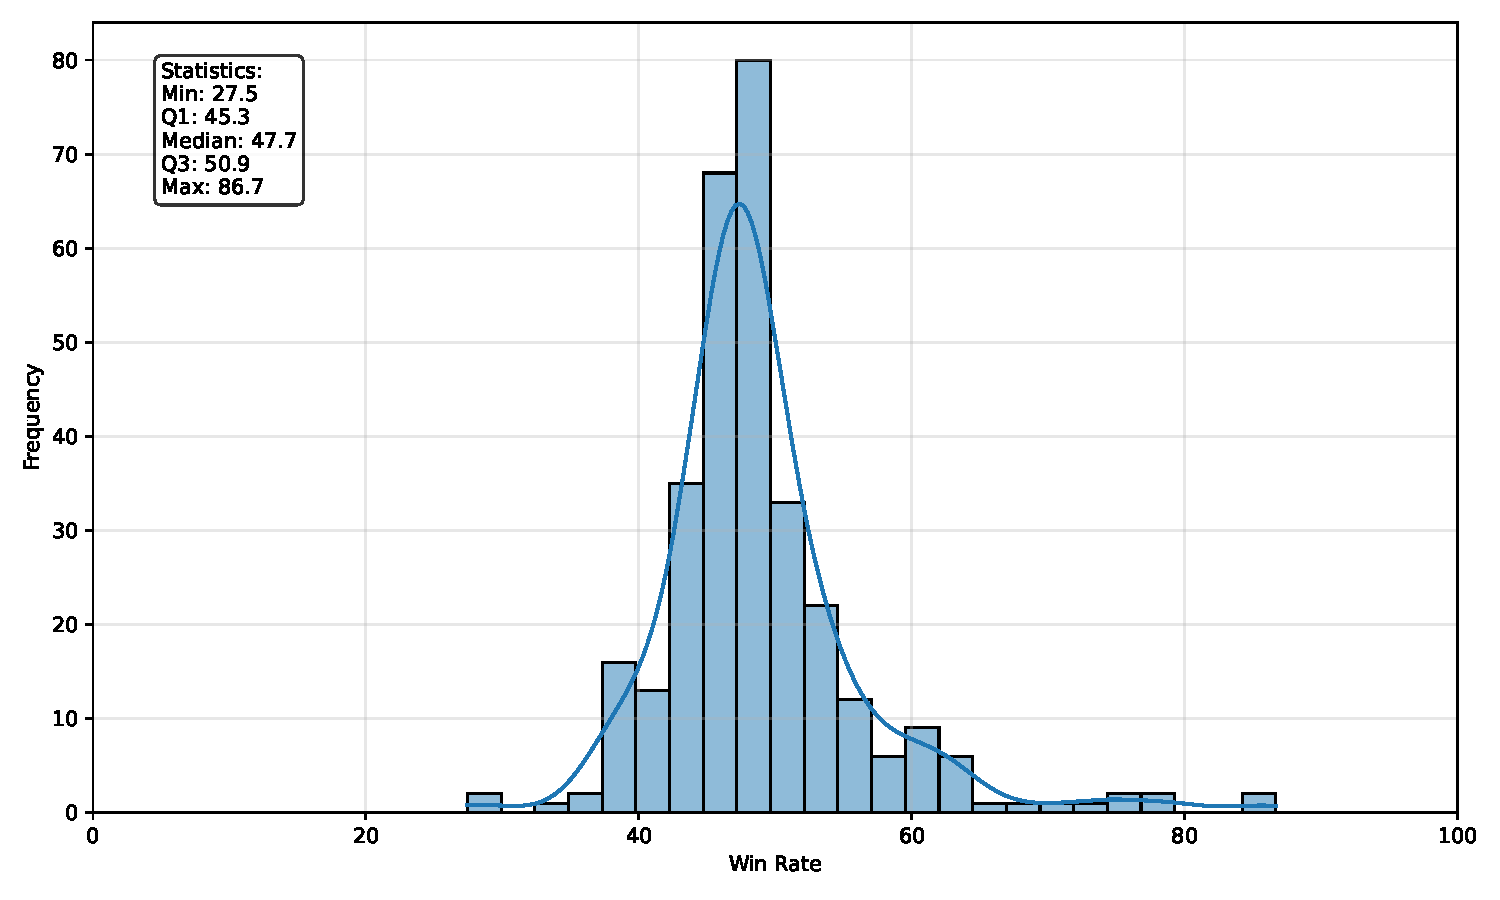
\includegraphics[width=0.8\textwidth]{../output/overall_win_rate_distribution.pdf} 
    \label{fig:overall_win_rate_histogram}
\end{figure}

Instead of career win rate, we can also look at annual win rates by wrestler. Figure \ref{fig:annual_win_rate_histogram} shows the distribution of annual win rates by wrestler-tournament from 2000 to 2025, along with summary statistics.\footnote{We filter out wrestlers with fewer than 45 total bouts.} The median annual win rate is 48.9\%, while the 25th and 75th percentiles are 44.9\% and 53.8\%, respectively. The distribution is again right-skewed, with a longer right tail of wrestlers with very high win rates. This distribution is wider than the career win rate distribution, which is expected since there is more variance in a single year (six tournaments) than over an entire career. In any case, this distribution still suggests that sumo wrestling is a highly competitive sport.

\begin{figure}[H]
    \centering
    \caption{Distribution of Annual Win Rates by Wrestler-Tournament (2000-2025)}
    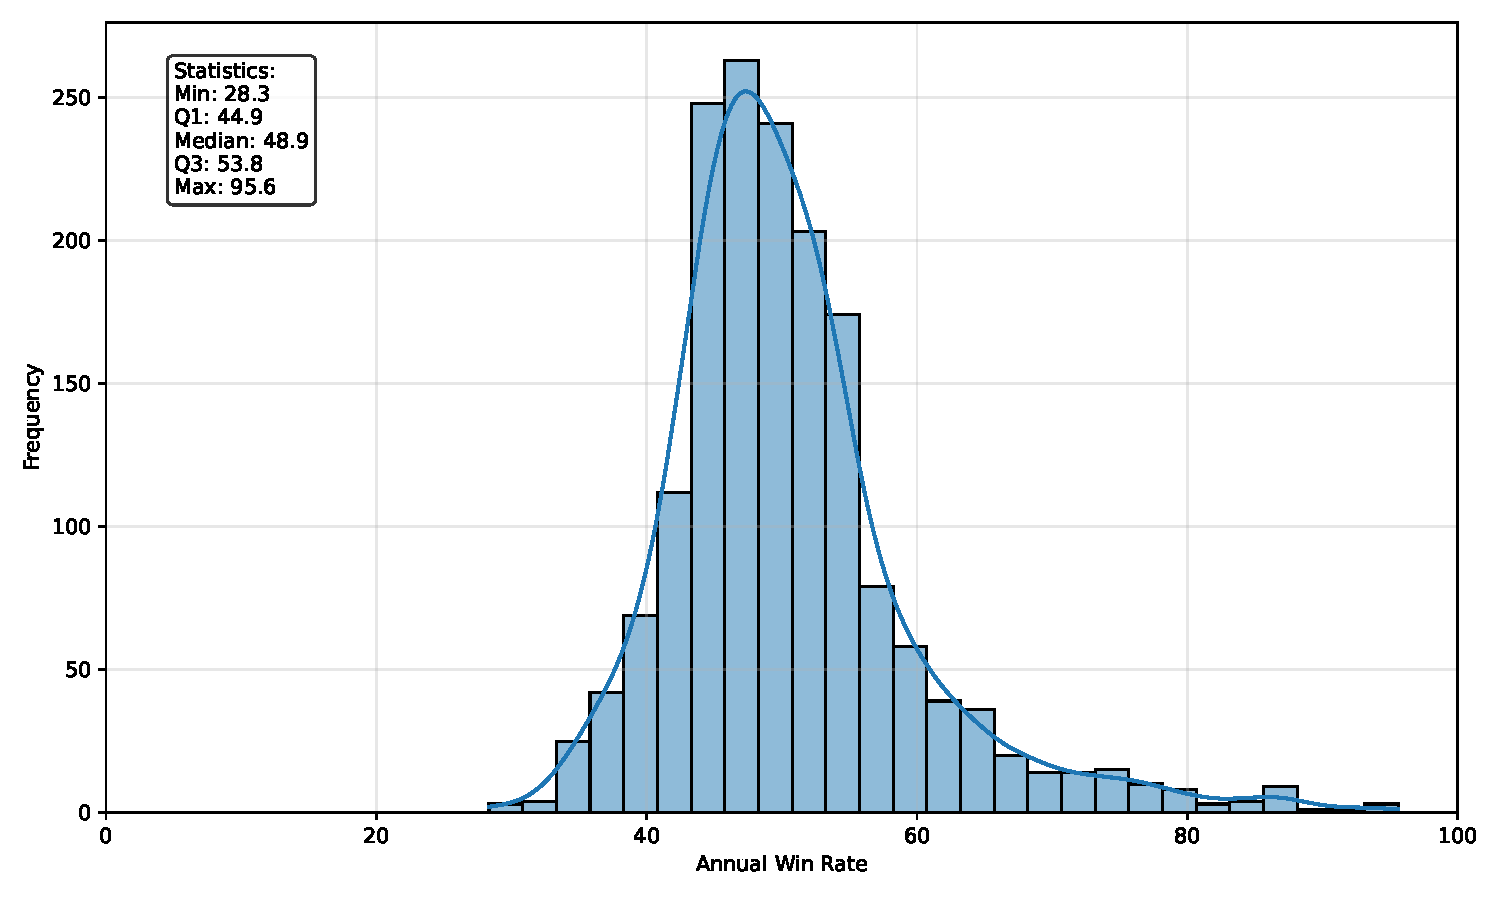
\includegraphics[width=0.8\textwidth]{../output/annual_win_rate_distribution.pdf} 
    \label{fig:annual_win_rate_histogram}
\end{figure}

One additional way to summarize the annual win rate distribution presented above is to count how many wrestlers have ever sustained a win rate above (or below) a certain threshold. For example, how many wrestlers had a year with a win rate 5\% above 50 (i.e. 55\%)? The table below summarizes various thresholds. We see that in a given year, fewer than 20\% of wrestlers will have a win rate above 60\% or below 40\%. This suggests that it is quite difficult to sustain a very high or very low win rate in a given year, which again suggests that sumo wrestling is a competitive sport.
\begin{table}[H]
\centering
\caption{Wrestler-Years with Sustained High or Low Win Rates (2000-2025)}
\begin{tabular}{lcc}
\toprule
Win Rate Differential & Count & \% \\
\midrule
Total &      1698 & 100\% \\
$\pm$ 5\%   & 786 & 46.3\% \\
$\pm$ 10\%  & 324 & 19.1\% \\
$\pm$ 15\%  & 132 & 7.8\% \\
$\pm$ 20\%  & 73  & 4.3\% \\
$\pm$ 25\%  & 44  & 2.6\% \\
\bottomrule
\end{tabular}
\end{table}

Now, we address the question of whether sumo is becoming more (or less) competitive over time. In Figure \ref{fig:std_win_rate_over_time}, we calculate the standard deviation of win rate within each tournament (across wrestlers), and then graph this standard deviation over time. We also fit a linear regression to the data to identify general trends. We find that while there is certainly variation in the standard deviation from tournament to tournament, there is essentially no trend over time. The slope of the fitted line is almost completely flat. This suggests that sumo wrestling has not undergone any sustained changes in competitiveness in the past 25 years.

\begin{figure}[H]
    \centering
    \caption{Standard Deviation of Win Rate by Tournament (2000-2025)}
    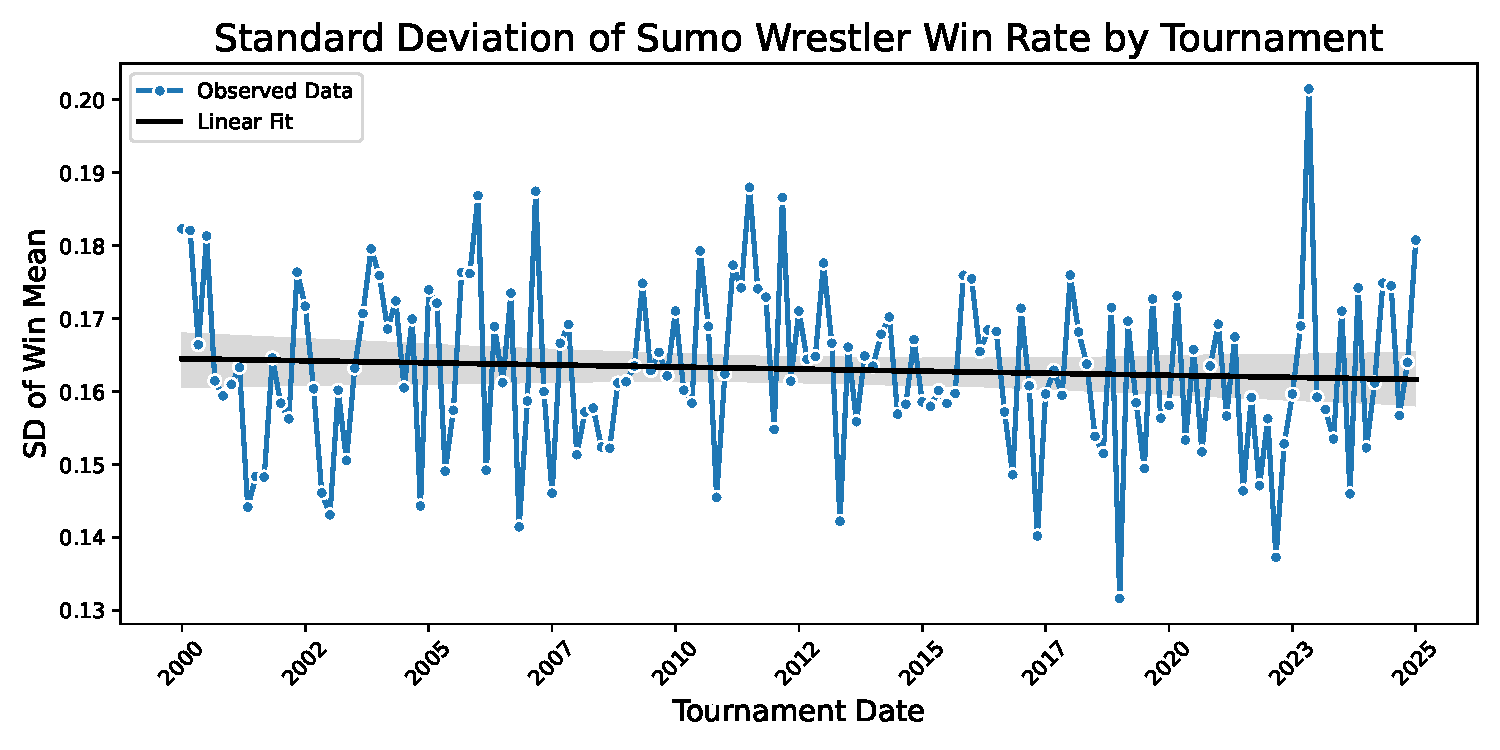
\includegraphics[width=0.9\textwidth]{../output/std_win_mean_by_tournament.pdf} 
    \label{fig:std_win_rate_over_time}
\end{figure}

So far, the analysis has shown that sumo is overall a competitive sport, and that it has not undergone any significant changes in competitiveness over the past 25 years. However, we have not touched on whether certain characteristics of the wrestler decide the outcome of each bout. Now, we turn to the question of how predictable sumo bouts are based on observable characteristics. We use two different models to analyze bout-level outcomes: a logistic regression model and a LightGBM model. First, we report our logit model results.

\begin{figure}[H]
    \centering
    \caption{Logit Model Results (Predicting Bout Outcomes)}
    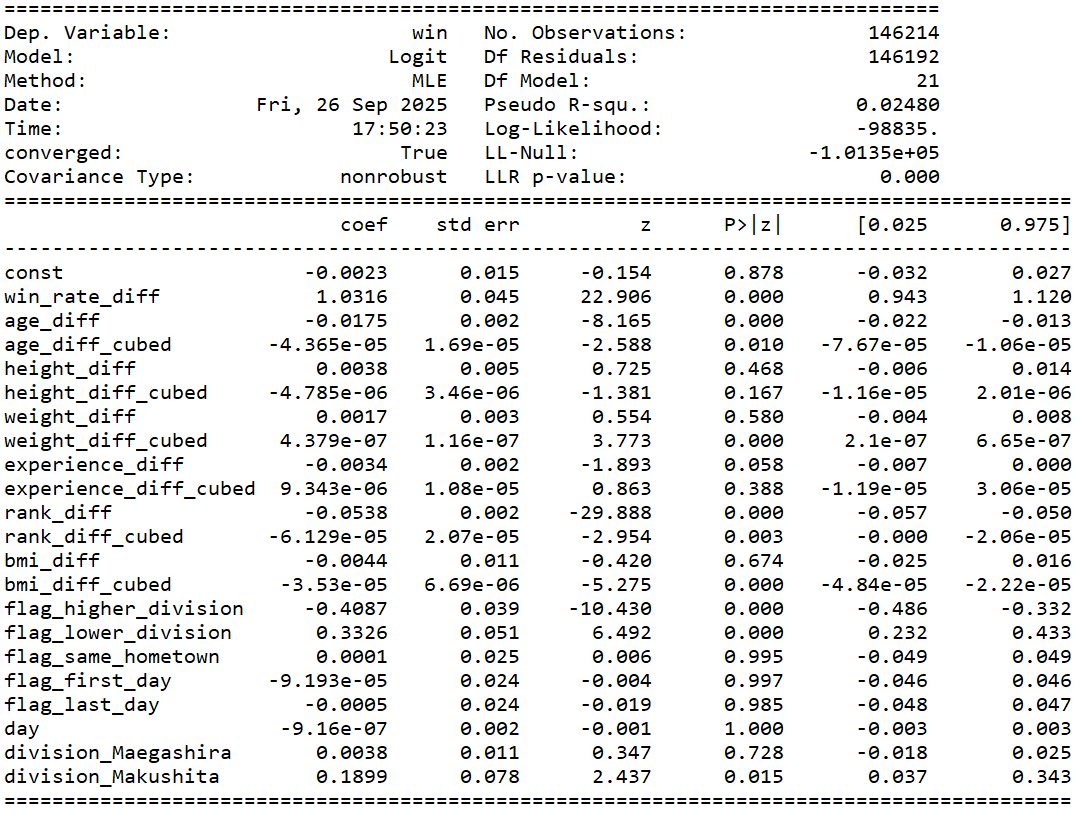
\includegraphics[width=0.9\textwidth]{../output/logit.png} 
    \label{fig:logit_model_results}
\end{figure}

The most obvious result from the logit model is that the difference in historical win rate is almost the exclusive factor that matters to the bout outcome. Win rate here is measured as a proportion, so a wrestler with a 10 percentage point historical win rate advantage has $\exp(0.1\cdot 1.0316) = 1.11$ odds of winning the bout (or a 52.6\% chance), a 20 percentage point advantage yields odds of 1.29 (55.1\% chance), and a 50 point advantage gives 1.67 odds (62.6\% chance). In other words, a wrestler with a 30\% historical win rate matched up against a wrestler with an 80\% historical win rate still has a 37.4\% chance of winning a particular bout, all else equal. These are certainly not decisive advantages at the bout level. Also note the extremely low pseudo $R^2$ of 0.025, which indicates that the model is very poor at predicting bout outcomes.

Additional controls in the regression yield useful insights. Holding win rate differential constant, height and weight differences have no bearing on bout outcomes, while younger wrestlers have a slight advantage on average. Wrestlers with a better rank (rank\_diff $< 0$) also have a slight expected advantage holding win rate differential constant. Interestingly, the coefficient on flag\_higher\_division, which identifies whether the wrestler is in a higher division than their opponent, is negative. This could be due to tournament organizers only arranging cross-division fights between the most promising prospects in the lower division and the worst performers in the higher division. 

As a last attempt to model bout outcomes, we use a LightGBM (gradient boosting tree) model, which allows for more complex relationships among the variables than the logit model. We train the LightGBM model on a 90\% random sample of the bouts, and test its performance on a 10\% holdout sample. If bouts are predictable based on observables, we should expect that the model has a high area under the receiver operating characteristic curve (AUC) on the test set. The AUC is a measure of how well the model can predict bout outcomes, with 0.5 being no better than random chance and 1 being perfect prediction. The LightGBM model achieves an AUC of 0.61 on the test set, which is better than random chance but not particularly high. This suggests that while some characteristics of the wrestlers do help predict bout outcomes, there is still a significant amount of unpredictability in sumo wrestling.\footnote{Alternative interpretations of these results are that we have omitted important variables that decide bout outcomes, and/or that fighter skill is an important factor that we are not controlling for.}

\begin{figure}[H]
    \centering
    \caption{LightGBM Model ROC Curve (Predicting Bout Outcomes)}
    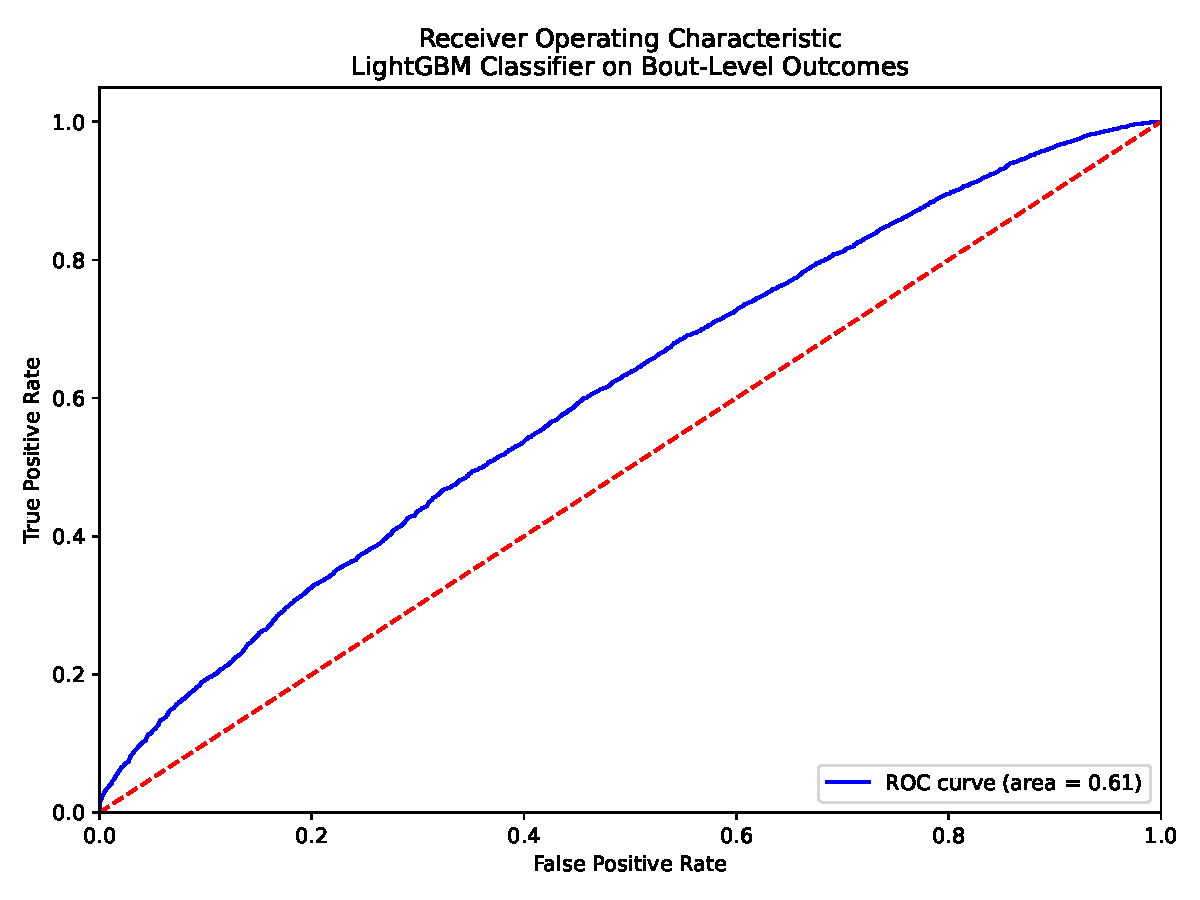
\includegraphics[width=0.8\textwidth]{../output/roc_curve_bout_level_model.pdf} 
    \label{fig:lightgbm_model_results}
\end{figure}

\section{Conclusion}
In this paper, we have analyzed the competitiveness of professional sumo wrestling over a period of 25 years. We find that sumo wrestling is overall a competitive sport, with most wrestlers having career win rates clustered around 50\%. We also find that there has been no significant change in the competitiveness of sumo wrestling over time. Finally, we find that while some characteristics of wrestlers do help predict bout outcomes, there is still a significant amount of unpredictability in sumo wrestling. Overall, our analysis suggests that sumo wrestling is a competitive and unpredictable sport.

\end{document}